\chapter{Kết quả}
\label{ch:results}

\section{Điều kiện đo}
Mọi số chu kỳ trong chương này là số chu kỳ đồng hồ của PicoRV32 trong mô phỏng RTL Verilator 5.032 của SoC (Mục~\ref{sec:latency} và Bảng~\ref{tab:socmap}), đo bằng lệnh \code{rdcycle} quanh đoạn mã cần đo. CPU và \NPU{} cùng một miền đồng hồ. Cấu hình PicoRV32: RV32IM, \code{ENABLE\_FAST\_MUL}, \code{BARREL\_SHIFTER}, không nén lệnh; RAM trả lời sau một chu kỳ. ``CPU-only'' là cùng firmware nhưng gọi \code{cpu\_matmul} thay cho \code{npu\_matmul}; mọi phần khác (im2col, pooling, cập nhật LSTM) giống hệt nhau. Hệ số tăng tốc (speedup) là tỉ số chu kỳ CPU-only trên chu kỳ CPU+\NPU{}. Nguồn số liệu: các tệp \code{results/*.log}.

\section{Độ chính xác}
\label{sec:res-acc}
Bảng~\ref{tab:accuracy} so sánh độ chính xác trên toàn bộ \num{10000} ảnh kiểm tra MNIST. Cột số thực lấy từ \code{model/README.txt}; cột INT8 là kết quả của mô hình số nguyên \code{cnn\_int}/\code{lstm\_int} trong \code{scripts/quantize.py}, vốn bit-exact với RTL trên mọi ảnh đã chạy trong mô phỏng (8 ảnh CNN, 16 ảnh LSTM, Chương~\ref{ch:verif}).

\begin{table}[H]
  \centering
  \caption{Độ chính xác trên \num{10000} ảnh kiểm tra MNIST}
  \label{tab:accuracy}
  \begin{tabular}{lccc}
    \toprule
    Mô hình & Float32 & INT8 (đường \NPU{}) & Chênh lệch (điểm \%) \\
    \midrule
    LeNet-5 & 98,83\% & 98,85\% & $+0{,}02$ \\
    LSTM ($T=28$, $F=28$, $H=16$) & 97,58\% & 97,50\% & $-0{,}08$ \\
    \bottomrule
  \end{tabular}
\end{table}

Lượng tử hóa sau huấn luyện INT8 theo tensor làm thay đổi độ chính xác dưới 0,1 điểm phần trăm cho cả hai mạng. Mức tăng $+0{,}02$ điểm của LeNet-5 (2 ảnh trên \num{10000}) nằm trong biên nhiễu thống kê và không nên hiểu là lượng tử hóa ``cải thiện'' mô hình. Mức giảm nhỏ của LSTM là đáng chú ý vì LSTM có đường hồi quy 28 bước, nơi sai số lượng tử có thể tích lũy; việc dùng LUT 256 phần tử cho sigmoid/tanh và trạng thái ô nhớ $c$ với độ phân giải $2^{-14}$ (Mục~\ref{sec:lstm-fixed}) đủ để kiểm soát sai số này. Trên 8 ảnh CNN và 16 ảnh LSTM chạy trong RTL, cả bản CPU và bản \NPU{} đều dự đoán đúng nhãn (8/8, 16/16).

\section{GEMM đơn lẻ}
\label{sec:res-gemm}
Bảng~\ref{tab:gemm} cho kết quả của \code{gemm\_demo}: nhân $(M\times N)\cdot(N\times N)$ một lần. Cột ``\NPU{} busy'' là giá trị thanh ghi CYCLES, khớp chính xác với công thức \eqref{eq:tbusy} $M+2N$.

\begin{table}[H]
  \centering
  \caption{GEMM đơn lẻ: chu kỳ CPU-only, tổng chu kỳ phía host khi dùng \NPU{}, và chu kỳ busy của \NPU{}}
  \label{tab:gemm}
  \begin{tabular}{rrrrrr}
    \toprule
    $N$ & $M$ & CPU-only & CPU+\NPU{} & \NPU{} busy & Speedup\\
    \midrule
    \multirow{4}{*}{4} & 1 & 785 & 883 & 9 & 0,89$\times$ \\
     & 8 & \num{6161} & \num{2456} & 16 & 2,51$\times$ \\
     & 32 & \num{24593} & \num{7803} & 40 & 3,15$\times$ \\
     & 64 & \num{49169} & \num{14945} & 72 & 3,29$\times$ \\
    \midrule
    \multirow{4}{*}{8} & 1 & \num{2785} & \num{1629} & 17 & 1,71$\times$ \\
     & 8 & \num{22133} & \num{4576} & 24 & 4,84$\times$ \\
     & 32 & \num{88469} & \num{14718} & 48 & 6,01$\times$ \\
     & 64 & \num{176917} & \num{28209} & 80 & 6,27$\times$ \\
    \bottomrule
  \end{tabular}

  \smallskip
  \raggedright\footnotesize Nguồn: \code{results/run\_N4.log} ($N=4$) và \code{results/gemm\_demo\_N8.log} ($N=8$). Tệp \code{results/run\_N8.log} chứa một lần chạy khác của cùng chương trình với tổng chu kỳ \NPU{} lớn hơn đúng 956 chu kỳ ở mọi $M$ (chu kỳ busy giống hệt); độ lệch hằng số này phù hợp với một phiên bản firmware cũ nạp trọng số chậm hơn, nên báo cáo dùng \code{gemm\_demo\_N8.log}.
\end{table}

Ba nhận xét: (i) với $M=64$, mảng chỉ bận 80 chu kỳ trong tổng số \num{28209} chu kỳ (0,28\%) -- phần còn lại là CPU ghi \num{16} từ trọng số, \num{128} từ kích hoạt, đọc \num{512} từ kết quả INT32 và polling; (ii) với $N=4$, $M=1$, dùng \NPU{} còn \emph{chậm hơn} CPU (0,89$\times$) vì chi phí điều khiển lớn hơn 16 phép MAC; (iii) speedup tăng theo $M$ do chi phí nạp trọng số được chia cho nhiều hàng -- đúng tinh thần của dataflow weight-stationary.

\section{LeNet-5}
\label{sec:res-cnn}
\subsection{Chu kỳ trên mỗi ảnh}
Bảng~\ref{tab:cnn-cycles} là trung bình trên 8 ảnh. Số chu kỳ gần như không phụ thuộc dữ liệu (chênh lệch giữa các ảnh dưới 0,03\%).

\begin{table}[H]
  \centering
  \caption{LeNet-5: chu kỳ trung bình trên mỗi ảnh (8 ảnh)}
  \label{tab:cnn-cycles}
  \begin{tabular}{lrr}
    \toprule
     & $N=4$ & $N=8$ \\
    \midrule
    CPU-only & \num{13235583} & \num{13254324} \\
    CPU + \NPU{} & \num{3427171} & \num{1923665} \\
    \textbf{Speedup} & \textbf{3,86$\times$} & \textbf{6,89$\times$} \\
    Số lượt chạy \NPU{} & \num{2964} & 741 \\
    Tổng chu kỳ busy của \NPU{} & \num{45402} & \num{17298} \\
    Busy / tổng thời gian \NPU{} & 1,32\% & 0,90\% \\
    Hiệu suất dùng mảng $\frac{\text{MAC}}{N^2\cdot\text{busy}}$ & 38,8\% & 25,4\% \\
    \bottomrule
  \end{tabular}
\end{table}

Số chu kỳ busy khớp chính xác với tổng của \eqref{eq:tbusy} trên mọi lượt chạy. Ví dụ với $N=8$: conv1 có $36$ lượt $M=64$ ($36\cdot80$) cộng 9 chu kỳ QUANT; conv2 $38\cdot80+2$; fc1 $480\cdot17+15$; fc2 $165\cdot17+11$; fc3 $22\cdot17+2$; tổng $\num{2889}+\num{3042}+\num{8175}+\num{2816}+376=\num{17298}$. Hiệu suất dùng mảng (25,4\% với $N=8$) thấp chủ yếu do ba lớp FC chạy với $M=1$: mỗi lượt tốn $2N+1=17$ chu kỳ cho chỉ một hàng.

Hình~\ref{fig:cycles} so sánh trực quan CPU-only và CPU+\NPU{} cho cả hai mạng.

\begin{figure}[H]
  \centering
  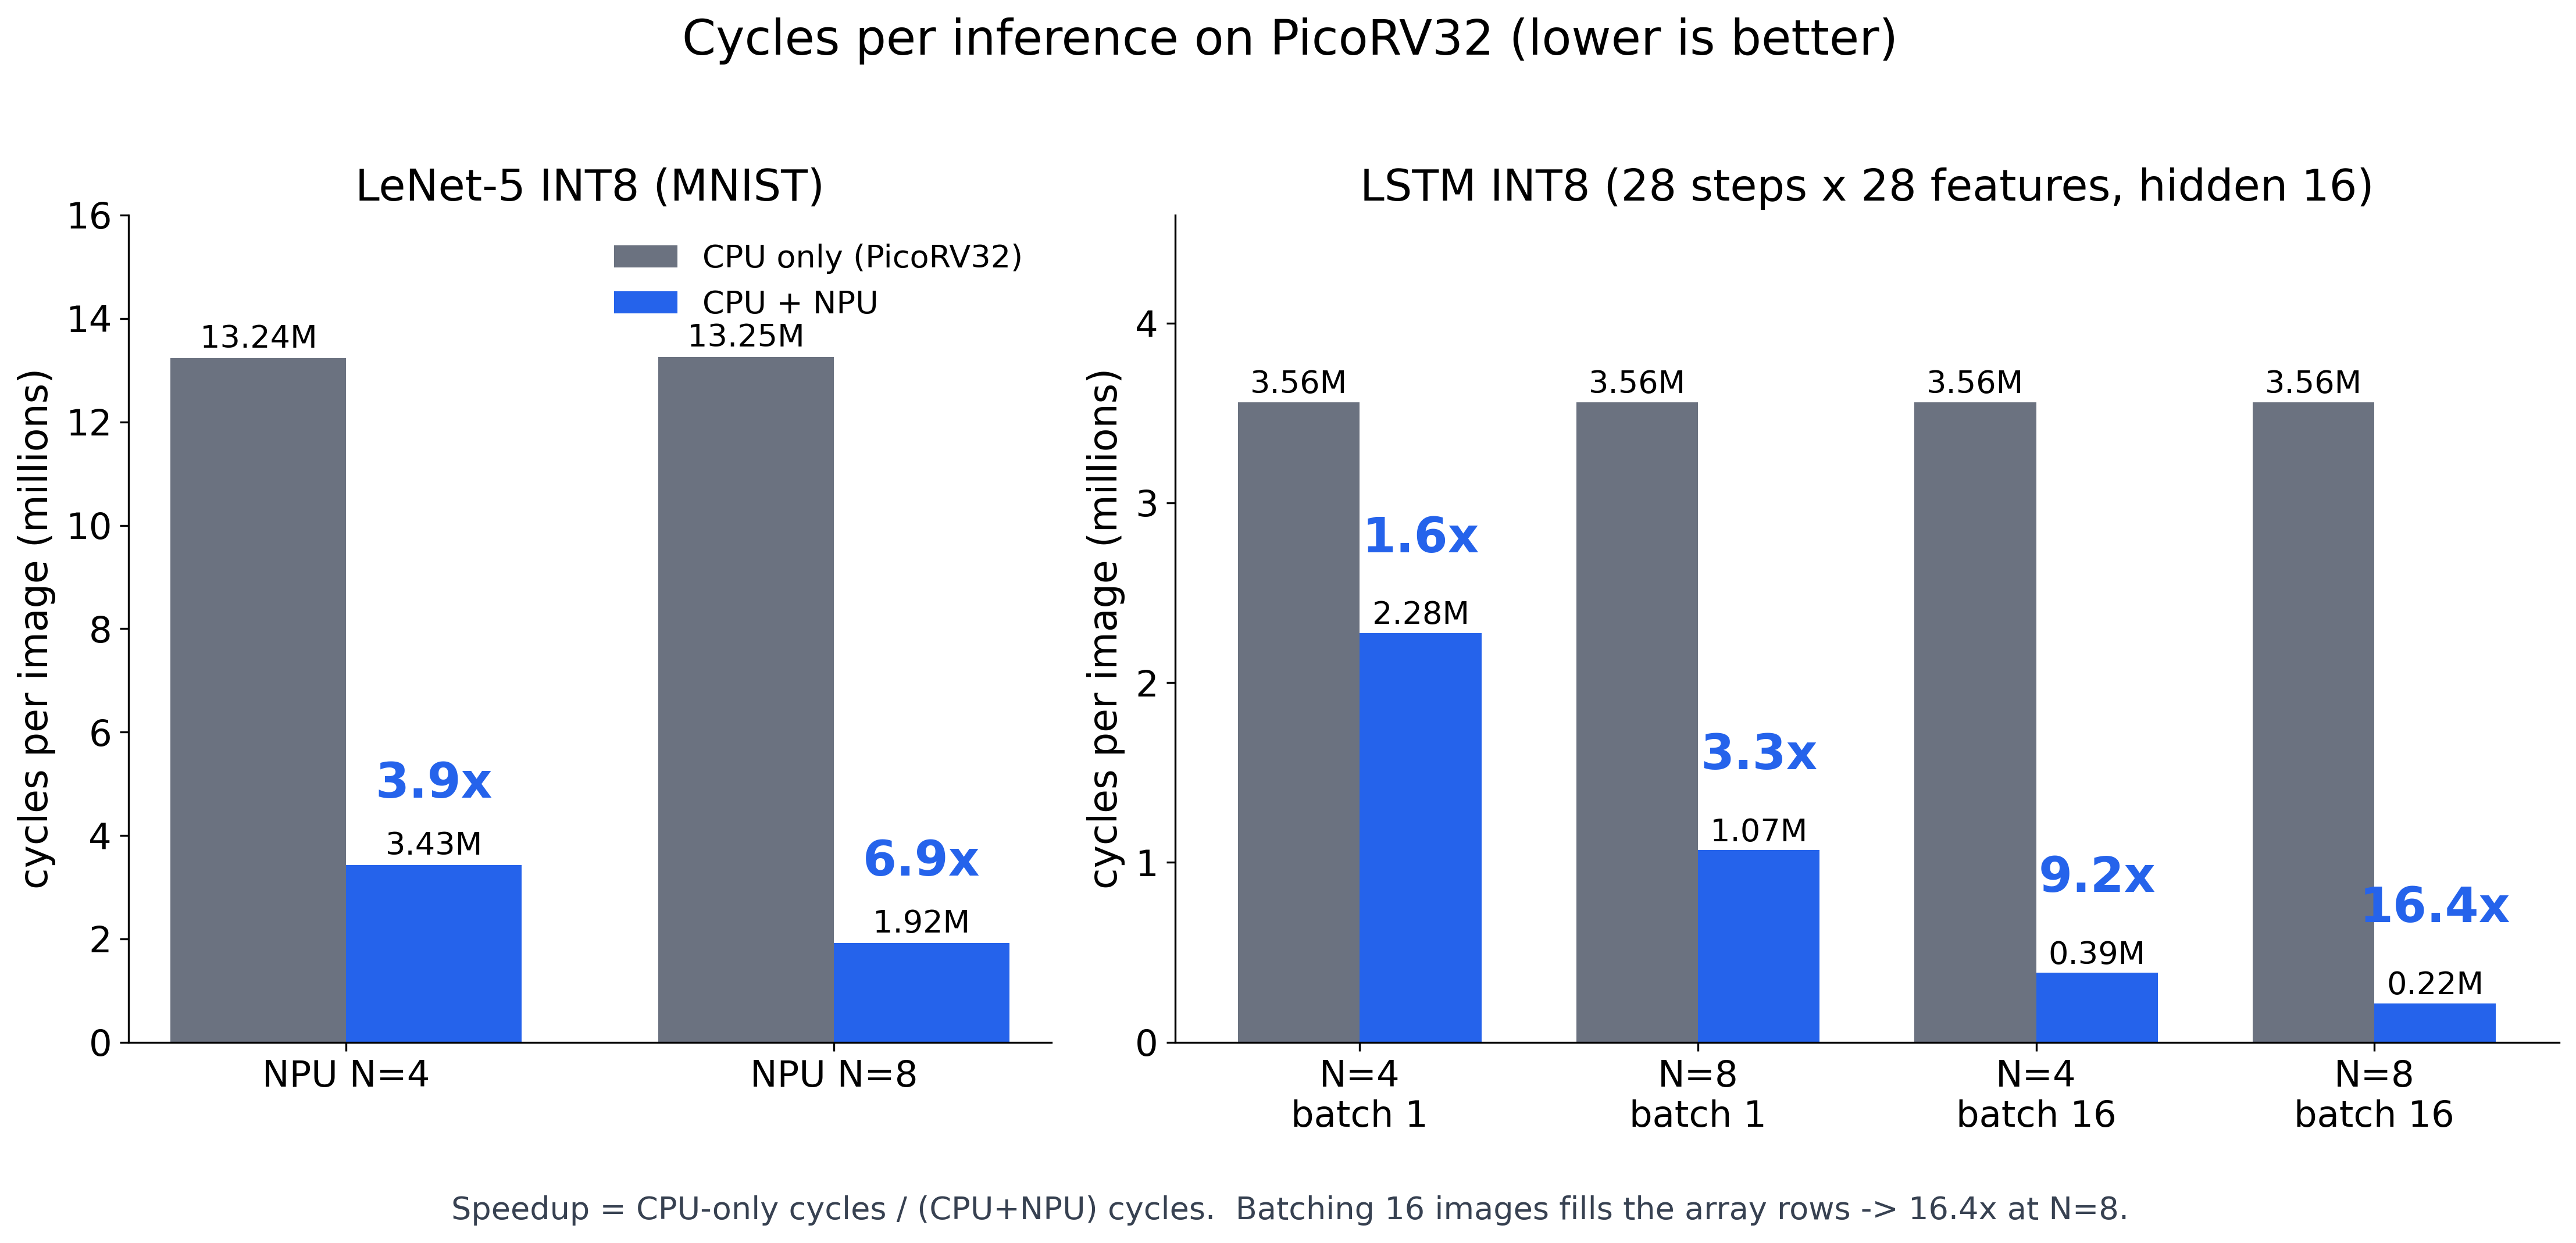
\includegraphics[width=\linewidth]{a_cycles_cpu_vs_npu.png}
  \caption{Chu kỳ trên mỗi ảnh trên PicoRV32 (thấp hơn là tốt hơn). Trái: LeNet-5; phải: LSTM với batch 1 và batch 16. Số liệu từ \code{results/cnn\_N*.log} và \code{results/lstm\_N*.log}.}
  \label{fig:cycles}
\end{figure}

\subsection{Phân tích profile và nút thắt}
\label{sec:profile}
Firmware đo thời gian theo pha bên trong \code{npu\_matmul} cho ảnh 0 (Bảng~\ref{tab:profile}, Hình~\ref{fig:profile}). ``Khác'' là phần còn lại của tổng thời gian: chuyển ảnh, im2col, maxpool, chi phí vòng lặp và gọi hàm.

\begin{table}[H]
  \centering
  \caption{Profile phía host của một ảnh LeNet-5 với \NPU{} (ảnh 0)}
  \label{tab:profile}
  \begin{tabular}{lrrrr}
    \toprule
    & \multicolumn{2}{c}{$N=4$} & \multicolumn{2}{c}{$N=8$}\\
    \cmidrule(lr){2-3}\cmidrule(lr){4-5}
    Pha & Chu kỳ & \% & Chu kỳ & \%\\
    \midrule
    Ghi trọng số & \num{524628} & 15,3 & \num{279357} & 14,5\\
    Ghi kích hoạt & \num{727524} & 21,2 & \num{257523} & 13,4\\
    Chạy + polling & \num{596100} & 17,4 & \num{141576} & 7,4\\
    Đọc kết quả & \num{54870} & 1,6 & \num{33291} & 1,7\\
    Khác (im2col, pool, \ldots) & \num{1524004} & 44,5 & \num{1211873} & 63,0\\
    \midrule
    Tổng & \num{3427126} & 100 & \num{1923620} & 100\\
    \bottomrule
  \end{tabular}
\end{table}

\begin{figure}[H]
  \centering
  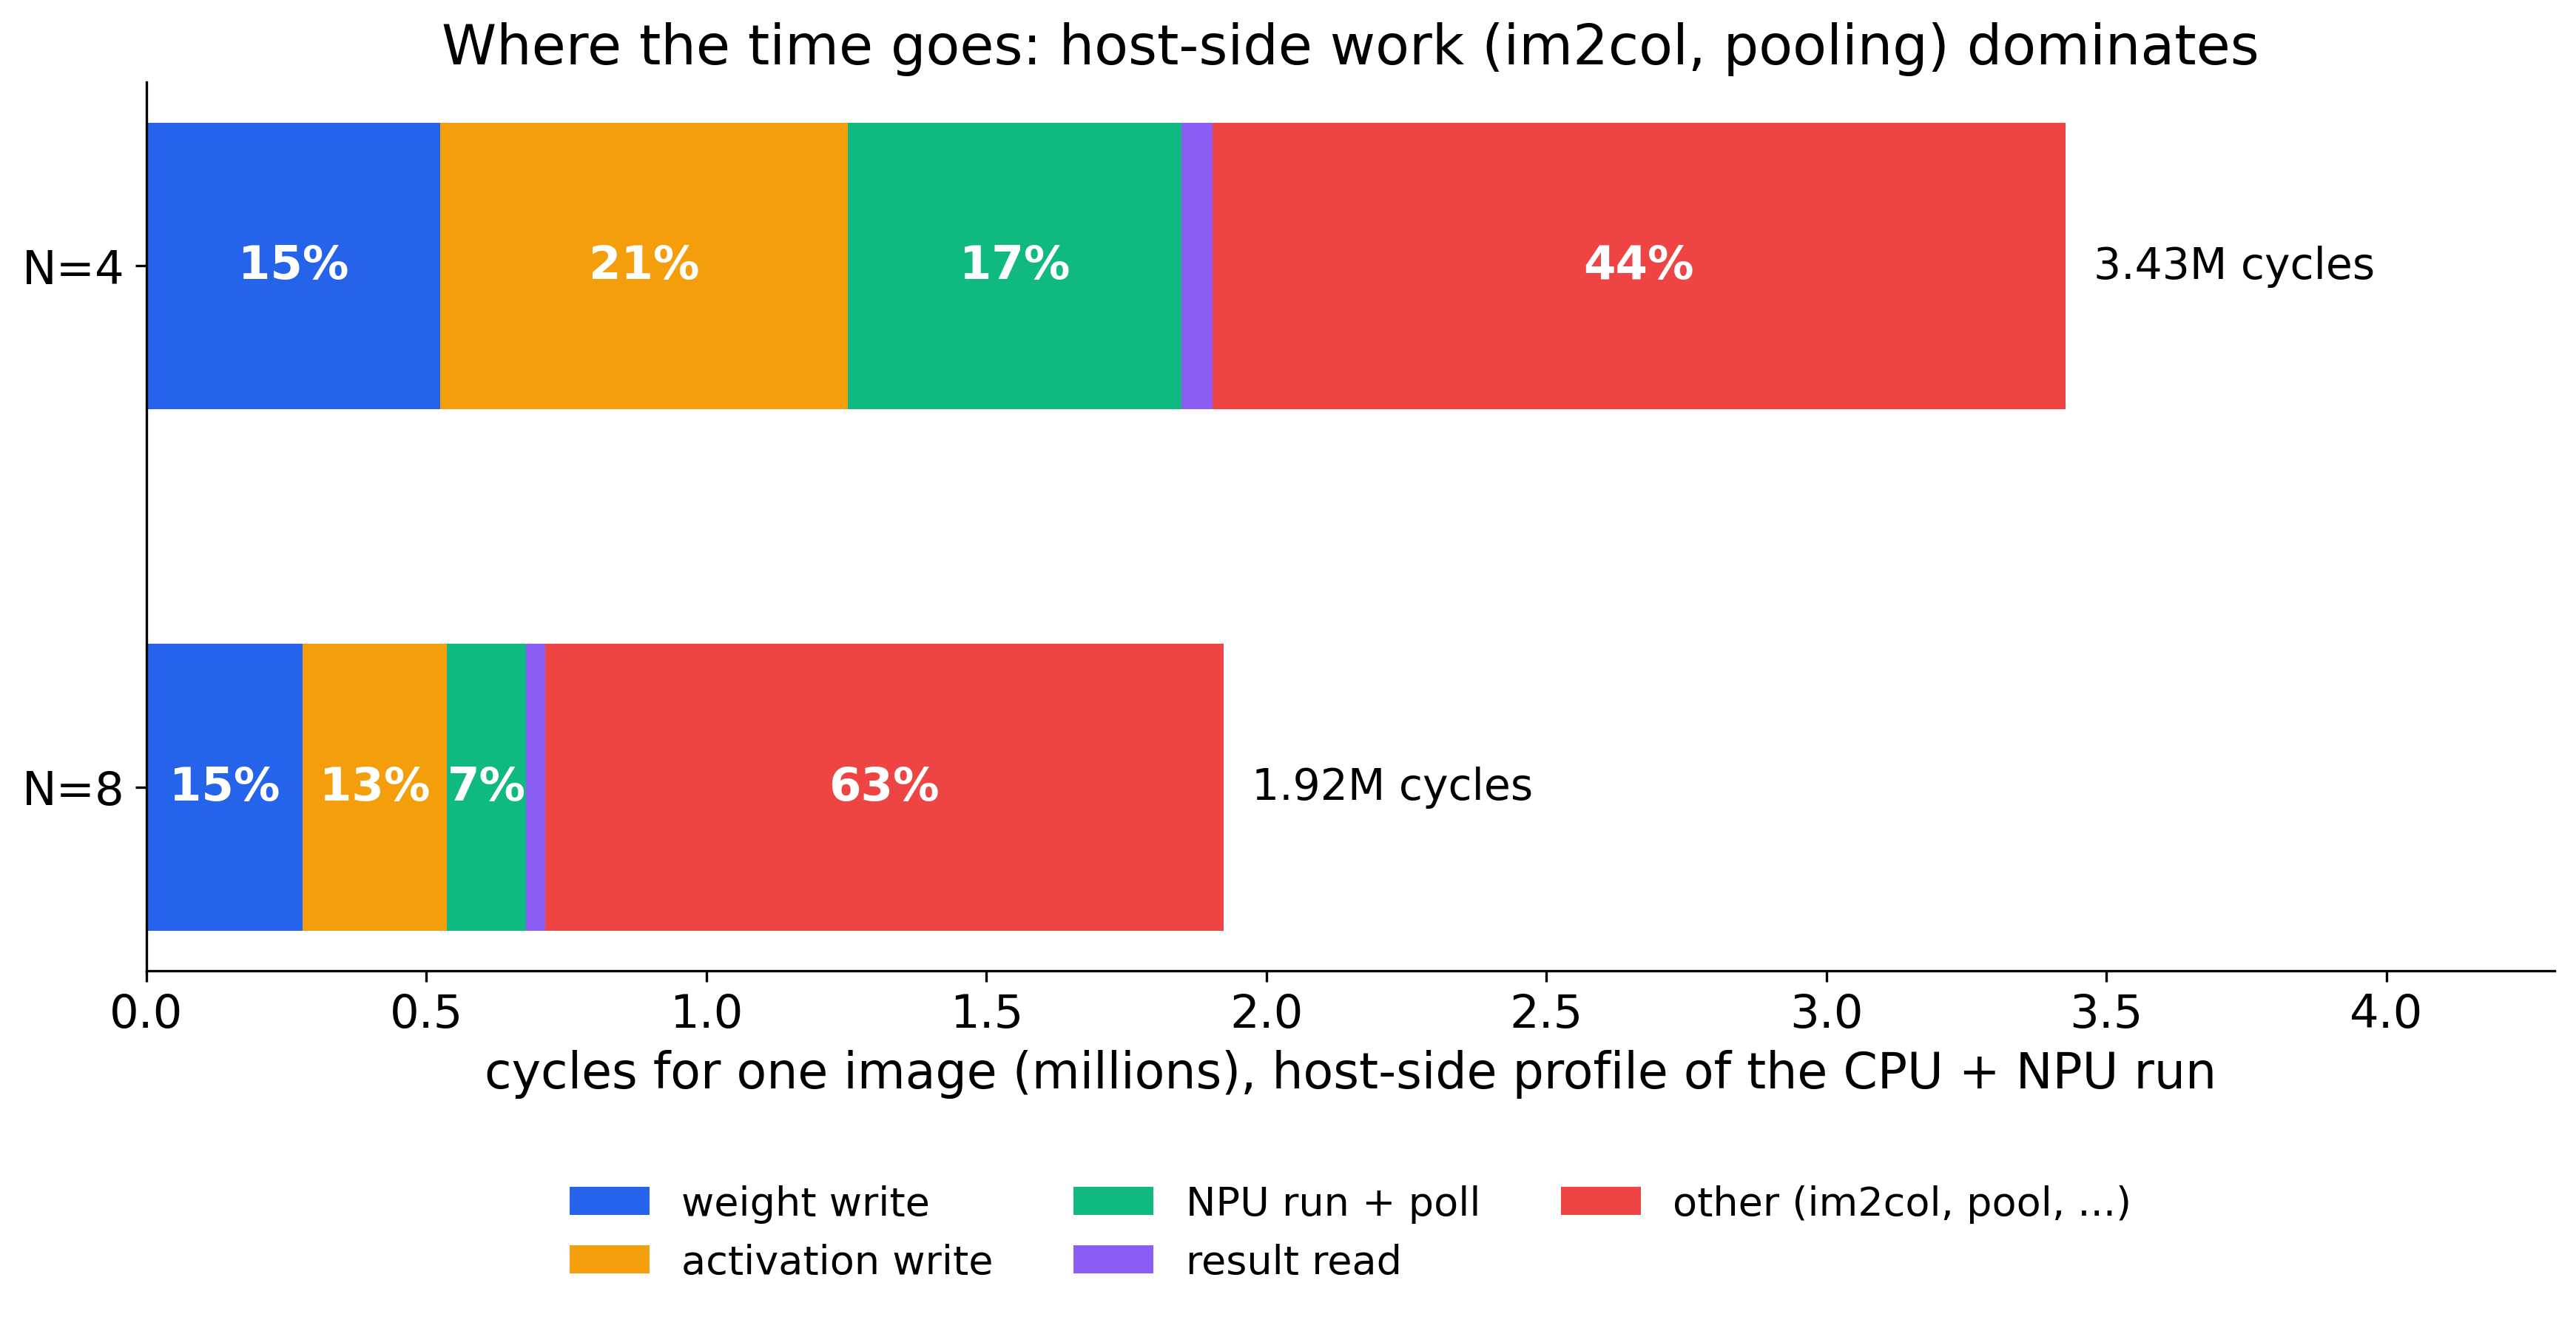
\includegraphics[width=\linewidth]{b_cnn_profile.png}
  \caption{Profile phía host của một ảnh LeNet-5: phần ``khác'' (im2col, pooling) chiếm ưu thế, đặc biệt với $N=8$.}
  \label{fig:profile}
\end{figure}

Các kết luận định lượng:
\begin{enumerate}
  \item \textbf{Mảng gần như rảnh rỗi.} Với $N=8$, mảng chỉ bận \num{17298} trên \num{1923620} chu kỳ (0,90\%). Pha ``chạy + polling'' trung bình $\num{141576}/741\approx191$ chu kỳ mỗi lượt, trong khi mảng bận trung bình $\num{17298}/741\approx23$ chu kỳ: phần lớn là chi phí MMIO (ghi M, CTRL; đọc STATUS, CYCLES; ghi CLEAR) của PicoRV32.
  \item \textbf{Chi phí truyền dữ liệu qua bus} (ghi trọng số, kích hoạt, đọc kết quả) là $\num{570171}$ chu kỳ (29,6\%) với $N=8$. Tính trung bình, mỗi lượt chạy tốn khoảng $(\num{279357}+\num{257523}+\num{141576}+\num{33291})/741\approx960$ chu kỳ phía host cho khoảng 23 chu kỳ tính.
  \item \textbf{Giới hạn Amdahl.} Phần ``khác'' (\num{1211873} chu kỳ với $N=8$) không được tăng tốc. Kể cả khi mọi pha liên quan tới \NPU{} tốn 0 chu kỳ, speedup tối đa với cách chia việc hiện tại là $\num{13254324}/\num{1211873}\approx10{,}9\times$. Muốn vượt giới hạn này phải đưa im2col và pooling xuống phần cứng (hoặc dùng DMA có hỗ trợ địa chỉ hóa kiểu im2col).
  \item Phần ``khác'' với $N=4$ lớn hơn với $N=8$ (\num{1524004} so với \num{1211873}) dù im2col và pooling giống nhau; chênh lệch khoảng \num{312000} chu kỳ này là chi phí vòng lặp và gọi hàm (bao gồm nạp bias/tham số requant, \code{rdcycle}) tỉ lệ với số lượt chạy (\num{2964} so với 741).
\end{enumerate}

\section{LSTM}
\label{sec:res-lstm}
Bảng~\ref{tab:lstm} tổng hợp kết quả LSTM (16 ảnh).

\begin{table}[H]
  \centering
  \caption{LSTM: chu kỳ trung bình trên mỗi ảnh}
  \label{tab:lstm}
  \begin{tabular}{lrrrr}
    \toprule
     & \multicolumn{2}{c}{$N=4$} & \multicolumn{2}{c}{$N=8$}\\
    \cmidrule(lr){2-3}\cmidrule(lr){4-5}
    Cấu hình & Chu kỳ/ảnh & Speedup & Chu kỳ/ảnh & Speedup\\
    \midrule
    CPU-only & \num{3559094} & 1,00$\times$ & \num{3559094} & 1,00$\times$ \\
    \NPU{}, batch 1 & \num{2275843} & 1,56$\times$ & \num{1068230} & 3,33$\times$ \\
    \NPU{}, batch 16 & \num{387103} & 9,19$\times$ & \num{217262} & 16,38$\times$ \\
    \midrule
    \NPU{} busy/ảnh, batch 1 & \num{48980} & & \num{23142} & \\
    \NPU{} busy/ảnh, batch 16 & \num{8116} & & \num{2710} & \\
    Lượt chạy/ảnh (batch 1) & \num{5392} & & \num{1348} & \\
    Hiệu suất dùng mảng, batch 1 & 10,1\% & & 5,3\% & \\
    Hiệu suất dùng mảng, batch 16 & 60,8\% & & 45,6\% & \\
    \bottomrule
  \end{tabular}
\end{table}

Với batch 1, LSTM chỉ đạt 3,33$\times$ ($N=8$) -- thấp hơn LeNet-5 -- vì mọi lượt chạy đều có $M=1$, giống lớp FC. Batching 16 ảnh làm mỗi lượt có $M=16$, nhờ đó cùng 1348 lượt chạy (với $N=8$) phục vụ 16 ảnh. Hiệu suất dùng mảng tăng từ 5,3\% lên 45,6\% và speedup tăng lên 16,38$\times$.

\subsection{Mô hình chi phí theo batch}
Khớp mô hình \eqref{eq:batchmodel} qua hai điểm đo $B=1$ và $B=16$ cho:
\begin{align}
  N=8:&\quad T_\text{fix}\approx\num{907699},\quad T_\text{var}\approx\num{160531} \text{ chu kỳ/ảnh},\\
  N=4:&\quad T_\text{fix}\approx\num{2014656},\quad T_\text{var}\approx\num{261187} \text{ chu kỳ/ảnh}.
\end{align}
Theo mô hình này, khi $B\to\infty$ speedup tiệm cận $\num{3559094}/T_\text{var}\approx22{,}2\times$ ($N=8$) và $13{,}6\times$ ($N=4$). Cần lưu ý: mô hình chỉ được khớp từ hai điểm và \emph{chưa được kiểm chứng} bằng các batch khác; ngoài ra $B$ bị giới hạn bởi DEPTH$=64$ hàng trong một lượt, và \code{run\_batch} hiện chỉ dùng tối đa \code{NIMG\_LSTM}$=16$. Phần $T_\text{var}$ gồm ghi kích hoạt, đọc kết quả và cập nhật element-wise trên CPU -- những phần không giảm theo batch.

\section{So sánh $N=4$ và $N=8$}
\label{sec:n4n8}
Tăng $N$ từ 4 lên 8 làm số MAC đỉnh tăng 4 lần (16 $\to$ 64 MAC/chu kỳ), số lượt chạy giảm 4 lần (vì cả khối $K$ và khối $C$ đều gấp đôi), độ trễ mỗi lượt tăng từ 8 lên 16 chu kỳ. Bảng~\ref{tab:n4n8} tóm tắt.

\begin{table}[H]
  \centering
  \caption{Ảnh hưởng của kích thước mảng $N$ (speedup so với CPU-only)}
  \label{tab:n4n8}
  \begin{tabular}{lccc}
    \toprule
    Workload & $N=4$ & $N=8$ & Tỉ số \\
    \midrule
    GEMM $M=64$ & 3,29$\times$ & 6,27$\times$ & 1,9 \\
    LeNet-5 & 3,86$\times$ & 6,89$\times$ & 1,8 \\
    LSTM batch 1 & 1,56$\times$ & 3,33$\times$ & 2,1 \\
    LSTM batch 16 & 9,19$\times$ & 16,38$\times$ & 1,8 \\
    \bottomrule
  \end{tabular}
\end{table}

Speedup chỉ tăng khoảng 1,8--2,1 lần chứ không phải 4 lần, vì thời gian bị chi phối bởi truyền dữ liệu và phần mềm, không phải bởi số MAC. Với $N$ lớn hơn nữa (16, 32), lợi ích sẽ tiếp tục giảm dần cho các mạng nhỏ như LeNet-5 trừ khi giải quyết được nút thắt truyền dữ liệu. Chi phí phần cứng tương ứng (diện tích, tài nguyên FPGA) được trình bày ở Chương~\ref{ch:fpga}.

\section{Ghi chú về chỉ số \code{npu\_busy\_share}}
Log CNN có trường \code{npu\_busy\_share\_x100} (132 với $N=4$, 89 với $N=8$). Trường này được tính bằng $\text{busy}\cdot\num{10000}/\text{tổng}$, tức là \emph{phần trăm nhân 100}: 132 nghĩa là 1,32\% và 89 nghĩa là 0,89\%, khớp với tỉ số busy/tổng trong Bảng~\ref{tab:cnn-cycles}. Hậu tố \code{\_x100} dễ bị đọc nhầm thành ``132\%''; báo cáo này không dùng trực tiếp trường đó mà tính lại tỉ số từ các cột \code{npu\_busy} và \code{npu\_cyc}.

\section{Tóm tắt}
\begin{itemize}
  \item Độ chính xác INT8 lệch dưới 0,1 điểm \% so với số thực; mọi đầu ra RTL bit-exact với golden.
  \item Với $N=8$: LeNet-5 nhanh hơn 6,9$\times$, LSTM 3,3$\times$ (batch 1) và 16,4$\times$ (batch 16) so với chỉ dùng PicoRV32.
  \item Mảng systolic bận dưới 1\% thời gian; nút thắt là im2col/pooling trên CPU (63\%) và truyền dữ liệu MMIO (khoảng 30\%).
\end{itemize}
